\documentclass[aspectratio=169]{beamer}
\usetheme{Madrid}
\usecolortheme{default}
\usepackage[utf8]{inputenc}
\usepackage[T5]{fontenc}
\usepackage{graphicx}
\usepackage{hyperref}
\usepackage{booktabs}
\usepackage{amsmath}
\usepackage{listings}
\usepackage{xcolor}

\definecolor{codegreen}{rgb}{0,0.6,0}
\definecolor{codegray}{rgb}{0.5,0.5,0.5}
\definecolor{codepurple}{rgb}{0.58,0,0.82}
\definecolor{backcolour}{rgb}{0.95,0.95,0.92}

\lstdefinestyle{mystyle}{
    backgroundcolor=\color{backcolour},   
    commentstyle=\color{codegreen},
    keywordstyle=\color{magenta},
    numberstyle=\tiny\color{codegray},
    stringstyle=\color{codepurple},
    basicstyle=\ttfamily\footnotesize,
    breakatwhitespace=false,         
    breaklines=true,                 
    captionpos=b,                    
    keepspaces=true,                 
    numbers=left,                    
    numbersep=5pt,                  
    showspaces=false,                
    showstringspaces=false,
    showtabs=false,                  
    tabsize=2
}
\lstset{style=mystyle}

\setbeamertemplate{caption}[numbered]
\renewcommand{\figurename}{Hình}
\renewcommand{\thefigure}{3.\arabic{figure}}

\title[Chương 3: Frameworks \& Keras]{Học Sâu (Deep Learning) \\ \vspace{0.5cm} \Large Chương 3: Giới thiệu TensorFlow, PyTorch, JAX và Keras}
\author{Đại học Đông Á}
\date{\today}

\begin{document}

\begin{frame}
    \titlepage
\end{frame}

\begin{frame}{Nội dung chương}
    \tableofcontents
\end{frame}

\section{1. Lịch sử phát triển các Framework Học sâu}

\begin{frame}{Kỷ nguyên khởi nguyên (Trước 2009)}
    \begin{itemize}
        \item Các nhà nghiên cứu phải tự viết tay logic tính toán đạo hàm (thường bằng C++).
        \item GPU programming gần như bất khả thi do chưa có kiến trúc hỗ trợ tốt.
        \item Năm 2006, NVIDIA phát hành CUDA, nhưng chủ yếu phục vụ mô phỏng vật lý chứ chưa phải Machine Learning.
    \end{itemize}
\end{frame}

\begin{frame}{Sự ra đời của các Framework đầu tiên (2009 - 2015)}
    \begin{itemize}
        \item \textbf{Theano (2009):} Framework đầu tiên hỗ trợ tự động tính đạo hàm (autograd) và tính toán GPU. Là "tổ tiên" của mọi framework hiện đại.
        \item Cuộc thi ImageNet 2012 làm bùng nổ sự quan tâm toàn cầu tới Deep Learning, thúc đẩy các framework như Torch 7 (Lua) và Caffe (C++).
        \item \textbf{Keras (Đầu 2015):} Ra mắt với tư cách là thư viện Deep Learning cấp cao, dễ sử dụng, được xây dựng trên nền Theano.
    \end{itemize}
\end{frame}

\begin{frame}{Kỷ nguyên hiện đại (Cuối 2015 - Nay)}
    \begin{itemize}
        \item \textbf{TensorFlow (Cuối 2015):} Do Google phát triển, hỗ trợ huấn luyện quy mô lớn (distributed computation).
        \item \textbf{PyTorch (Cuối 2016):} Do Meta (Facebook) phát triển để đối trọng, nổi bật với tính linh hoạt (Dynamic Computation Graph).
        \item \textbf{JAX (2018):} Một hệ thống gọn nhẹ từ Google kết hợp Autograd và trình biên dịch XLA, tối ưu vô cùng mạnh mẽ cho GPU/TPU.
    \end{itemize}
\end{frame}

\begin{frame}{Ba tính năng cốt lõi của một Framework}
    Để huấn luyện Deep Learning hiện đại, mọi framework (TF, PyTorch, JAX) đều phải giải quyết tốt 3 bài toán:
    \begin{enumerate}
        \item Khả năng tự động tính đạo hàm cho các hàm phức tạp (Auto-differentiation).
        \item Khả năng tính toán số học tensor cực nhanh trên GPU/TPU thay vì CPU.
        \item Khả năng phân tán tính toán trên nhiều thiết bị (Multi-GPU/TPU) hoặc nhiều máy tính.
    \end{enumerate}
\end{frame}

\begin{frame}{Tương lai của hệ sinh thái Frameworks}
    \begin{itemize}
        \item Ngôn ngữ lập trình: Python thống trị hoàn toàn.
        \item Chúng ta đang sống trong thế giới Đa-Framework (Multi-framework): TF, PyTorch, JAX đều có chỗ đứng riêng.
        \item \textbf{Giá trị của Keras 3.0:} Giúp nhà phát triển chỉ cần viết mã một lần (Keras API), có thể linh hoạt chuyển đổi backend chạy trên bất kỳ framework nào (TF, Torch, JAX).
    \end{itemize}
\end{frame}

\section{2. Tổng quan về TensorFlow}

\begin{frame}{Giới thiệu TensorFlow}
    \begin{itemize}
        \item Là một hệ sinh thái mã nguồn mở (open-source) đồ sộ của Google.
        \item \textbf{Hệ sinh thái Enterprise (Doanh nghiệp):} Gồm TFX (quản lý workflow), TF Serving (triển khai API), TF Lite (di động), TensorFlow.js (trình duyệt).
        \item Phù hợp cho việc đưa sản phẩm AI ra môi trường thực tế (Production-grade).
    \end{itemize}
\end{frame}

\begin{frame}[fragile]{Tensors và Variables trong TensorFlow}
    Tensors là hằng số (không thể gán lại giá trị).
    \begin{lstlisting}[language=Python]
import tensorflow as tf
# Khoi tao hang so
x = tf.ones(shape=(2, 1))
y = tf.zeros(shape=(2, 1))
z = tf.constant([1, 2, 3], dtype="float32")

# Khoi tao ngau nhien
r1 = tf.random.normal(shape=(3, 1), mean=0., stddev=1.)
r2 = tf.random.uniform(shape=(3, 1), minval=0., maxval=1.)
    \end{lstlisting}
\end{frame}

\begin{frame}[fragile]{Sử dụng tf.Variable}
    TensorFlow tensors là \textit{không thể gán} (immutable). Để huấn luyện (cập nhật trọng số), ta phải dùng \textbf{Variable}.
    \begin{lstlisting}[language=Python]
v = tf.Variable(initial_value=tf.random.normal(shape=(3, 1)))

# Cap nhat gia tri
v.assign(tf.ones((3, 1)))
v[0, 0].assign(3.)

# Cap nhat cong/tru (nhu +=, -=)
v.assign_add(tf.ones((3, 1)))
v.assign_sub(tf.ones((3, 1)))
    \end{lstlisting}
\end{frame}

\begin{frame}[fragile]{Toán học Tensor (Operations) trong TensorFlow}
    \begin{lstlisting}[language=Python]
a = tf.ones((2, 2))
b = tf.square(a)  # Binh phuong
c = tf.sqrt(a)    # Can bac 2
d = b + c         # Cong tung phan tu (element-wise)

# Nhan ma tran (Dot product / Matmul)
e = tf.matmul(a, b)

# Ghep noi (Concatenate)
f = tf.concat((a, b), axis=0)
    \end{lstlisting}
\end{frame}

\begin{frame}[fragile]{Tự động tính đạo hàm với GradientTape}
    \begin{lstlisting}[language=Python]
input_var = tf.Variable(initial_value=3.0)
with tf.GradientTape() as tape:
    result = tf.square(input_var) # y = x^2
    
# Dao ham cua x^2 tai x=3 la 2*3 = 6
gradient = tape.gradient(result, input_var)
print(gradient) # Tra ve 6.0
    \end{lstlisting}
    \textit{Lưu ý:} GradientTape mặc định chỉ theo dõi (watch) các \texttt{tf.Variable} có khả năng huấn luyện.
\end{frame}

\begin{frame}[fragile]{Đạo hàm cấp 2 với TensorFlow}
    Chúng ta có thể lồng các GradientTape để tính đạo hàm cấp cao (vd: vận tốc $\rightarrow$ gia tốc).
    \begin{lstlisting}[language=Python]
time = tf.Variable(0.0)
with tf.GradientTape() as outer_tape:
    with tf.GradientTape() as inner_tape:
        position = 4.9 * time**2
    speed = inner_tape.gradient(position, time)
    
acceleration = outer_tape.gradient(speed, time) # 9.8
    \end{lstlisting}
\end{frame}

\begin{frame}[fragile]{Biên dịch để tăng tốc (Just-In-Time Compilation)}
    Thực thi mặc định của Python (Eager Execution) khá chậm. Có thể dùng \texttt{@tf.function} để biên dịch hàm Python thành một Computation Graph (Đồ thị tính toán) tối ưu bằng XLA:
    \begin{lstlisting}[language=Python]
@tf.function(jit_compile=True)
def dense(inputs, W, b):
    return tf.nn.relu(tf.matmul(inputs, W) + b)
    \end{lstlisting}
    \textit{Ưu điểm:} Cực nhanh. \textit{Nhược điểm:} Khó debug hơn vì mã chạy không còn là Python nguyên bản.
\end{frame}

\section{3. Tổng quan về PyTorch}

\begin{frame}{Giới thiệu PyTorch}
    \begin{itemize}
        \item \textbf{Thống trị mảng Nghiên cứu (Research):} Hơn 70\% các bài báo khoa học AI mới đều sử dụng PyTorch do sự thân thiện với lập trình viên (Pythonic).
        \item \textbf{Tính Pythonic cao:} Cú pháp rất gần gũi với NumPy.
        \item \textbf{Đồ thị tính toán Động (Dynamic Computation Graph):} Đồ thị được xây dựng on-the-fly, cực dễ chèn các lệnh \texttt{print} để debug.
    \end{itemize}
\end{frame}

\begin{frame}[fragile]{Tensors trong PyTorch}
    \begin{lstlisting}[language=Python]
import torch

# Khoi tao
x = torch.ones(size=(2, 1))
y = torch.zeros(size=(2, 1))
z = torch.tensor([1, 2, 3], dtype=torch.float32)

# Random (cu phap hoi khac biet)
r1 = torch.normal(mean=torch.zeros((3,1)), std=torch.ones((3,1)))
r2 = torch.rand(3, 1) # Uniform
    \end{lstlisting}
\end{frame}

\begin{frame}[fragile]{Gán Tensor và nn.Parameter}
    Khác với TF, PyTorch Tensors có thể trực tiếp gán giá trị:
    \begin{lstlisting}[language=Python]
x = torch.zeros(size=(2, 1))
x[0, 0] = 1.
    \end{lstlisting}
    Nhưng để theo dõi đạo hàm, ta sử dụng thuộc tính \texttt{requires\_grad=True}:
    \begin{lstlisting}[language=Python]
v = torch.ones(size=(3, 1), requires_grad=True)
# Hoac su dung Parameter khi viet Module
import torch.nn as nn
w = nn.Parameter(torch.rand(3, 3))
    \end{lstlisting}
\end{frame}

\begin{frame}[fragile]{Tính toán Gradient bằng .backward()}
    Cú pháp đạo hàm của PyTorch đơn giản hơn (không cần context manager GradientTape):
    \begin{lstlisting}[language=Python]
x = torch.tensor(3.0, requires_grad=True)
result = torch.square(x)

# Goi backward de tinh dao ham cho toan bo graph
result.backward()

# Xem dao ham cua result theo x
print(x.grad) # 6.0
    \end{lstlisting}
\end{frame}

\begin{frame}[fragile]{Tổ chức code với nn.Module}
    \begin{lstlisting}[language=Python]
class SimpleDense(nn.Module):
    def __init__(self, in_channels, out_channels):
        super().__init__()
        self.W = nn.Parameter(torch.rand(in_channels, out_channels))
        self.b = nn.Parameter(torch.zeros(out_channels))
        
    def forward(self, x):
        return torch.relu(torch.matmul(x, self.W) + self.b)
        
model = SimpleDense(64, 32)
    \end{lstlisting}
\end{frame}

\section{4. Tổng quan về JAX}

\begin{frame}{Giới thiệu JAX}
    \begin{itemize}
        \item JAX = Numpy + Autograd + XLA (Trình biên dịch tăng tốc cực độ).
        \item Phổ biến ở Google DeepMind, Midjourney, Anthropic do khả năng chạy cực lớn trên cụm TPU.
        \item \textbf{Lập trình hàm không trạng thái (Stateless):} Mọi hàm đều trong suốt (pure functions), không sử dụng biến toàn cục. Giúp JAX an toàn khi chạy song song.
    \end{itemize}
\end{frame}

\begin{frame}[fragile]{jax.numpy và PRNG Keys}
    JAX tái tạo 99\% API của Numpy thông qua \texttt{jax.numpy}:
    \begin{lstlisting}[language=Python]
from jax import numpy as jnp
x = jnp.ones(shape=(2, 1))
    \end{lstlisting}
    \textbf{PRNG Keys (Số ngẫu nhiên không trạng thái):}
    \begin{lstlisting}[language=Python]
import jax
# Phai tao "chia khoa" (key) de random
seed_key = jax.random.key(1337)
r1 = jax.random.normal(seed_key, shape=(3,))

# De lay random tiep theo, phai tao key moi
new_key = jax.random.split(seed_key, num=1)[0]
    \end{lstlisting}
\end{frame}

\begin{frame}[fragile]{Gán Tensor trong JAX}
    Giống TensorFlow, JAX tensor không thể gán trực tiếp. Phải dùng cú pháp \texttt{.at[].set()} để trả về một tensor mới:
    \begin{lstlisting}[language=Python]
x = jnp.array([1, 2, 3], dtype="float32")
# x[0] = 10 se bao loi
new_x = x.at[0].set(10)
    \end{lstlisting}
\end{frame}

\begin{frame}[fragile]{Tính toán Gradient bằng jax.grad()}
    JAX sử dụng phương pháp "siêu lập trình" (hàm trả về hàm) để tính đạo hàm:
    \begin{lstlisting}[language=Python]
def compute_loss(input_var):
    return jnp.square(input_var)

# Truyen ham loss qua jax.grad de lay ham tinh dao ham
grad_fn = jax.grad(compute_loss)

x = jnp.array(3.0)
print(grad_fn(x)) # 6.0
    \end{lstlisting}
\end{frame}

\begin{frame}[fragile]{Trả về cả Loss và Gradient}
    Thực tế, ta thường cần cả giá trị Loss và cấu trúc Gradient. JAX cung cấp \texttt{value\_and\_grad()}:
    \begin{lstlisting}[language=Python]
def compute_loss(state, x, y):
    # state co the la tuple (W, b)
    pass
    
# Tra ve mot ham moi
grad_fn = jax.value_and_grad(compute_loss)

# Tinh toan dong thoi
loss, grads = grad_fn(state, x, y)
    \end{lstlisting}
\end{frame}

\begin{frame}[fragile]{Biên dịch hàm cực nhanh với @jax.jit}
    \begin{lstlisting}[language=Python]
@jax.jit
def dense(inputs, W, b):
    return jax.nn.relu(jnp.matmul(inputs, W) + b)
    \end{lstlisting}
    \begin{itemize}
        \item JAX biên dịch hàm này thành mã máy XLA.
        \item \textit{Ràng buộc:} Hàm phải phi trạng thái (không sửa đổi biến ngoài, cập nhật tensor phải trả về).
    \end{itemize}
\end{frame}

\section{5. Mối quan hệ giữa Keras và các Backend}

\begin{frame}{Keras: High-Level API cho Deep Learning}
    \begin{itemize}
        \item Keras ra đời (2015) để giúp lập trình Deep Learning giống như chơi "lắp ghép LEGO".
        \item Keras che đi toàn bộ sự phức tạp của Low-level API (viết Gradient, vòng lặp lặp).
        \item Được sử dụng bởi Google, Netflix, Uber, Waymo.
    \end{itemize}
\end{frame}

\begin{frame}{Kiến trúc đa Backend của Keras}
    \begin{figure}
        \centering
        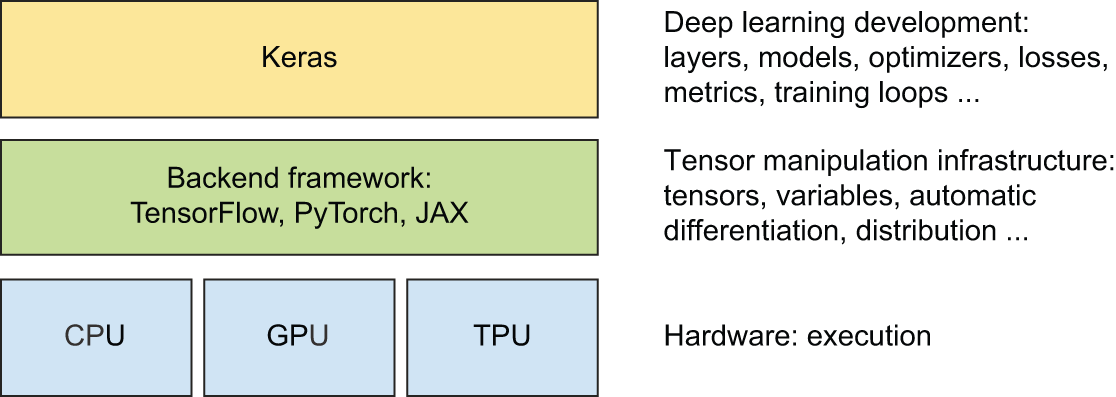
\includegraphics[width=\textwidth,height=0.7\textheight,keepaspectratio]{../../images/ch03/keras_and_backends.7fcf768f.png}
        \caption{Cấu trúc đa Backend của Keras 3.0}
    \end{figure}
\end{frame}

\begin{frame}[fragile]{Layer cơ sở: Thiết kế theo hướng Đối tượng}
    Trong Keras, \texttt{Layer} là khối xây dựng cơ bản, gồm trạng thái (weights) và tính toán (forward pass).
    \begin{lstlisting}[language=Python]
import keras
class SimpleDense(keras.Layer):
    def __init__(self, units):
        super().__init__()
        self.units = units
        
    def build(self, input_shape): # Goi 1 lan duy nhat
        self.W = self.add_weight(shape=(input_shape[-1], self.units))
        self.b = self.add_weight(shape=(self.units,))
        
    def call(self, inputs): # Thuc thi tinh toan
        return keras.ops.matmul(inputs, self.W) + self.b
    \end{lstlisting}
\end{frame}

\begin{frame}[fragile]{Lợi ích của hàm build()}
    Hàm \texttt{build()} cho phép Keras \textbf{tự động suy diễn hình dạng (shape inference)}. Bạn không cần chỉ định đầu vào dài bao nhiêu:
    \begin{lstlisting}[language=Python]
# Ban khong can quan tam lop truoc truyen vao bao nhieu unit
model = keras.Sequential([
    SimpleDense(32), # Tu dong hieu input_shape o day la 784
    SimpleDense(64),
    SimpleDense(10)
])
# Goi model tren du lieu thuc te se kich hoat build() hang loat
    \end{lstlisting}
\end{frame}

\begin{frame}[fragile]{Biên dịch Mô hình (model.compile)}
    Để cấu hình quá trình học tập, Keras có bước \texttt{compile} cực kỳ chuẩn hóa:
    \begin{lstlisting}[language=Python]
model.compile(
    optimizer="adam",     # Phep toi uu gradient descent
    loss="mse",           # Ham mat mat
    metrics=["accuracy"]  # Do do hieu suat hien thi
)
# Train tren du lieu
model.fit(x_train, y_train, epochs=10)
    \end{lstlisting}
\end{frame}

\section{6. Bài toán cốt lõi: Bộ Phân loại Tuyến tính}

\begin{frame}{Ôn tập toán học: Đường thẳng và Siêu phẳng}
    Mục tiêu: Xây dựng bộ phân loại tuyến tính (Linear Classifier) từ con số 0 để hiểu cơ chế lõi của học sâu.
    \begin{itemize}
        \item Phương trình dự đoán tổng quát (Hàm tuyến tính affine):
        \begin{equation}
            \mathbf{y\_pred} = \mathbf{W} \cdot \mathbf{x} + \mathbf{b}
        \end{equation}
        \item $\mathbf{W}$ (Trọng số - Weights): Quyết định độ nghiêng/hướng của đường thẳng.
        \item $\mathbf{b}$ (Độ lệch - Bias): Quyết định vị trí tịnh tiến của đường thẳng so với gốc toạ độ.
    \end{itemize}
\end{frame}

\begin{frame}{Khởi tạo dữ liệu giả lập (Point Clouds)}
    \begin{columns}
        \column{0.5\textwidth}
        Tạo 2 cụm điểm phân bố ngẫu nhiên trong không gian 2D:
        \begin{itemize}
            \item \textbf{Cụm 1:} Nhãn (label) = 0.
            \item \textbf{Cụm 2:} Nhãn (label) = 1.
        \end{itemize}
        Bài toán: Vẽ một đường thẳng tách biệt chính xác 2 cụm điểm này bằng Gradient Descent.
        
        \column{0.5\textwidth}
        \begin{figure}
            \centering
            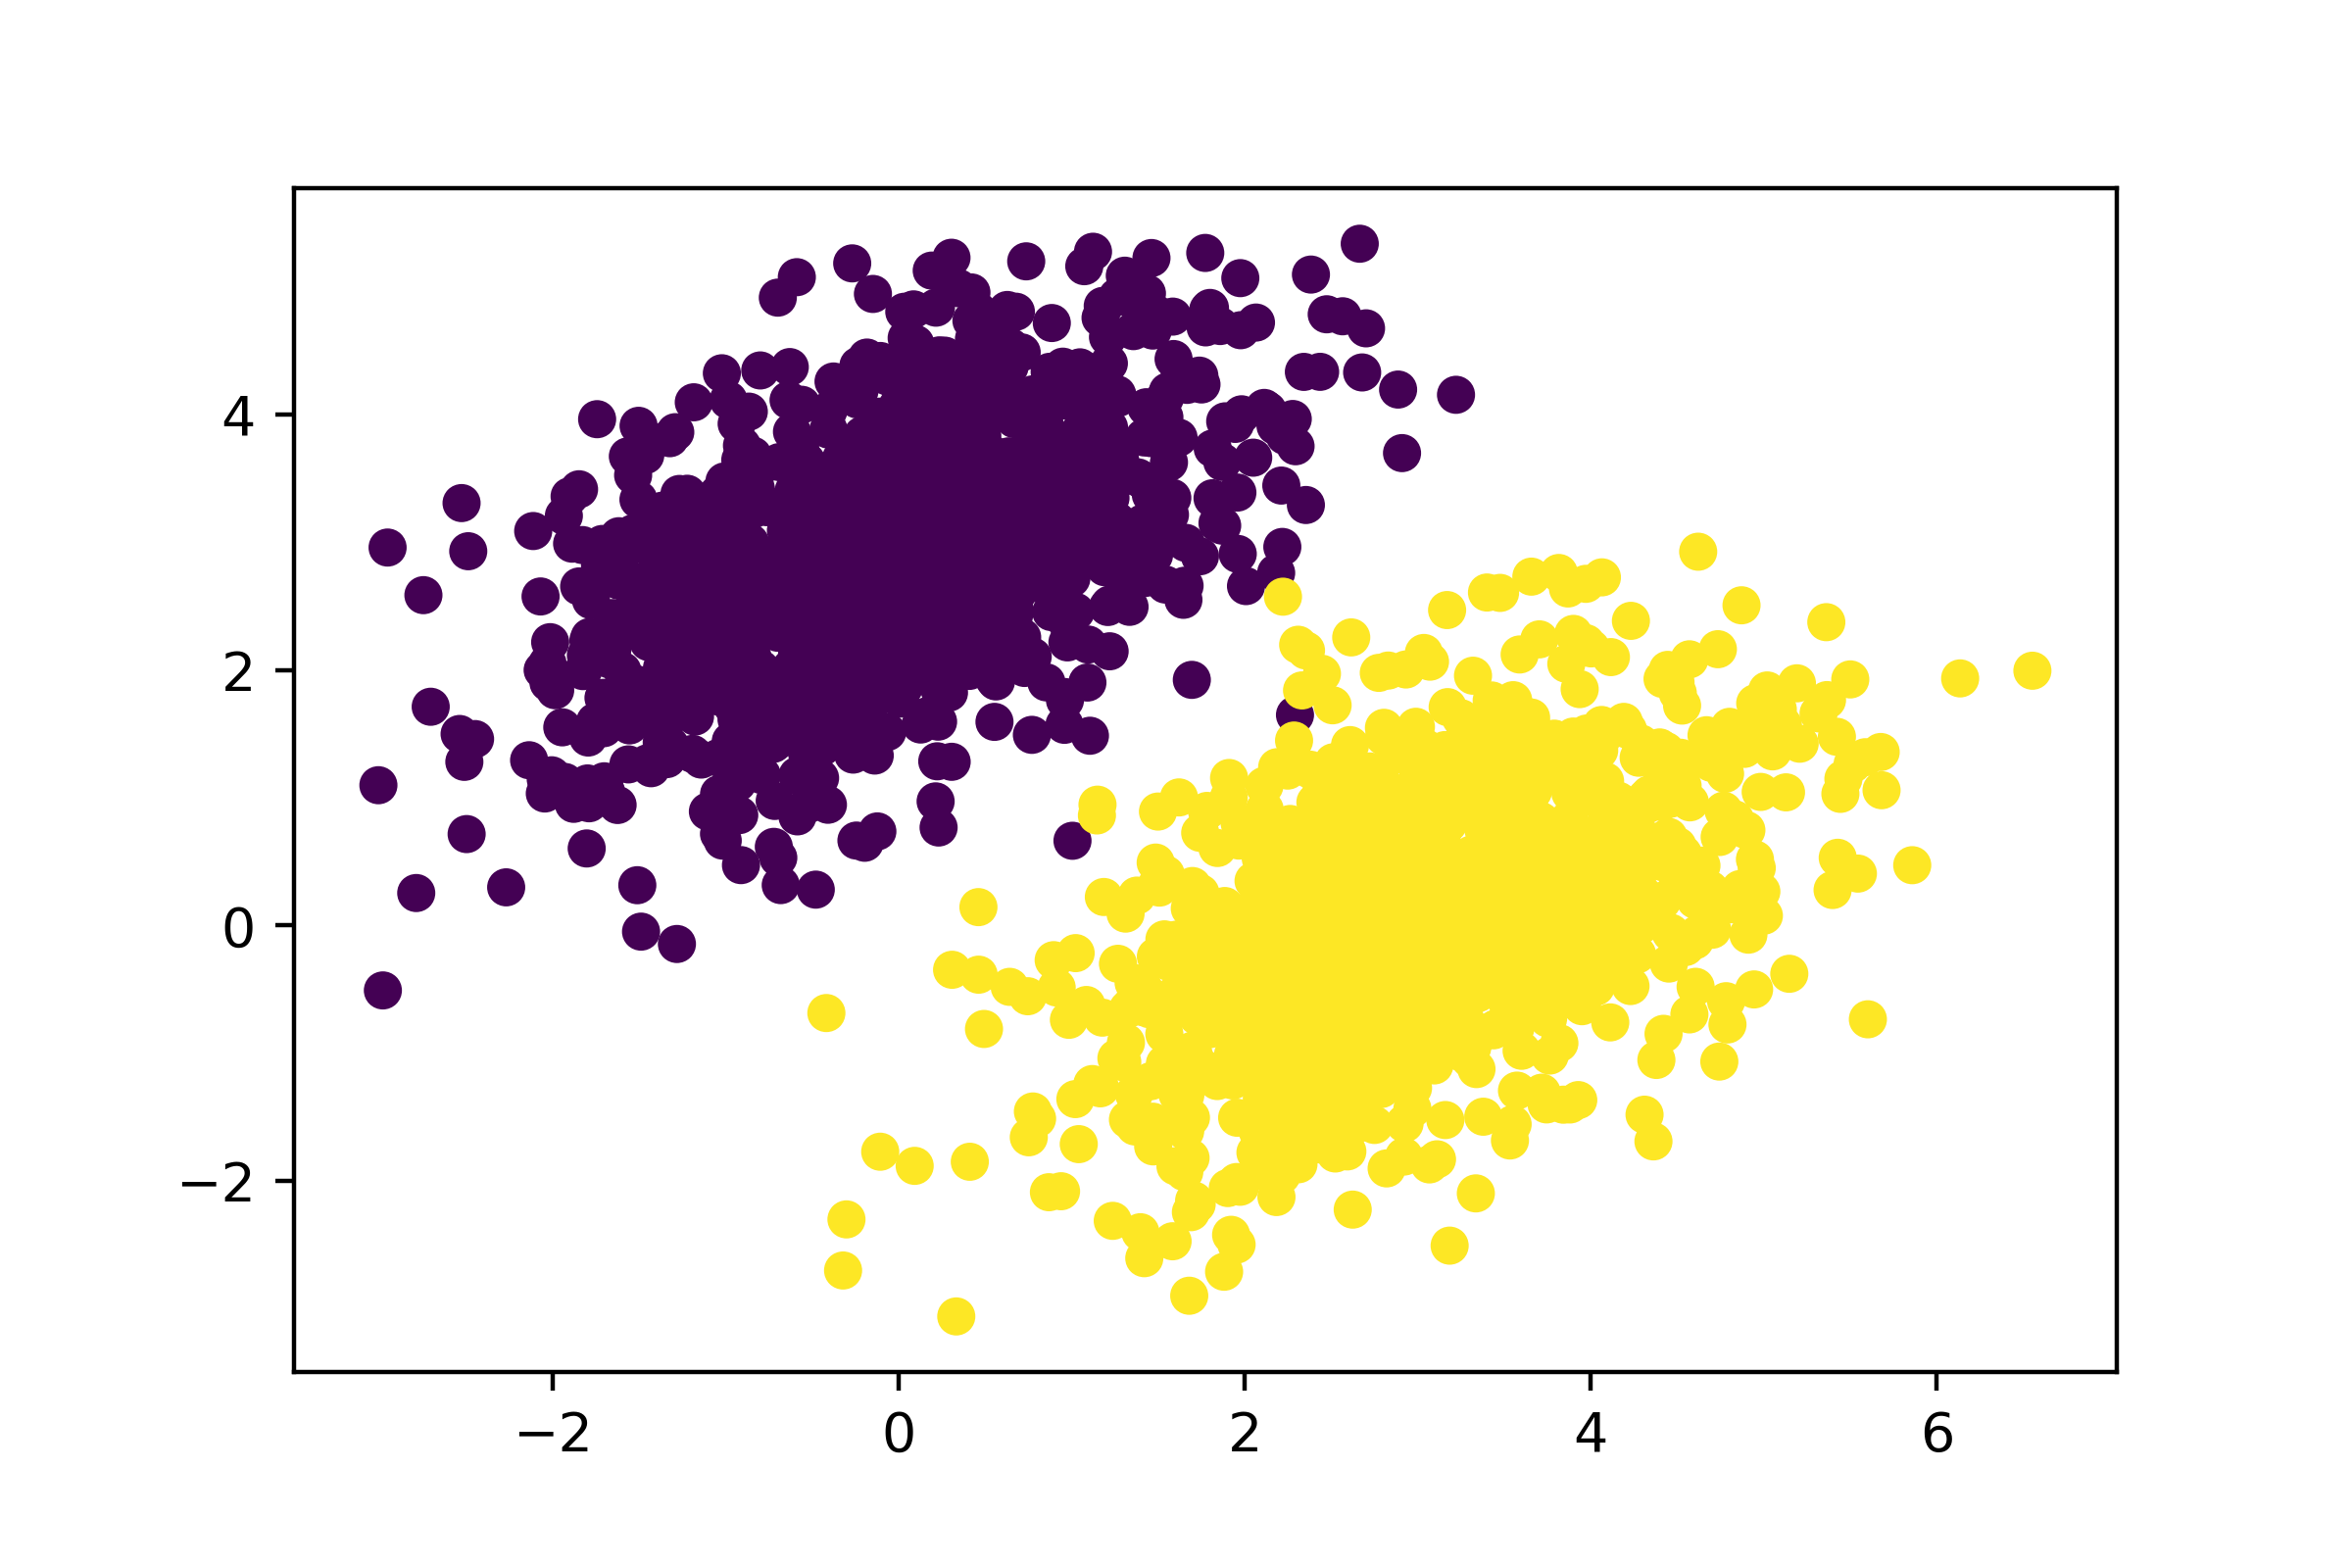
\includegraphics[width=\textwidth,height=0.7\textheight,keepaspectratio]{../../images/ch03/linear_model_inputs.282fc3b6.png}
            \caption{Hai cụm điểm dữ liệu ngẫu nhiên}
        \end{figure}
    \end{columns}
\end{frame}

\begin{frame}{Dự đoán ban đầu (Khởi tạo ngẫu nhiên)}
    \begin{columns}
        \column{0.5\textwidth}
        Khi mô hình phân loại vừa được tạo ra:
        \begin{itemize}
            \item $W, b$ ngẫu nhiên rất nhỏ (gần 0).
            \item Đường thẳng vô nghĩa, điểm MSE Loss rất cao.
        \end{itemize}
        
        \column{0.5\textwidth}
        \begin{figure}
            \centering
            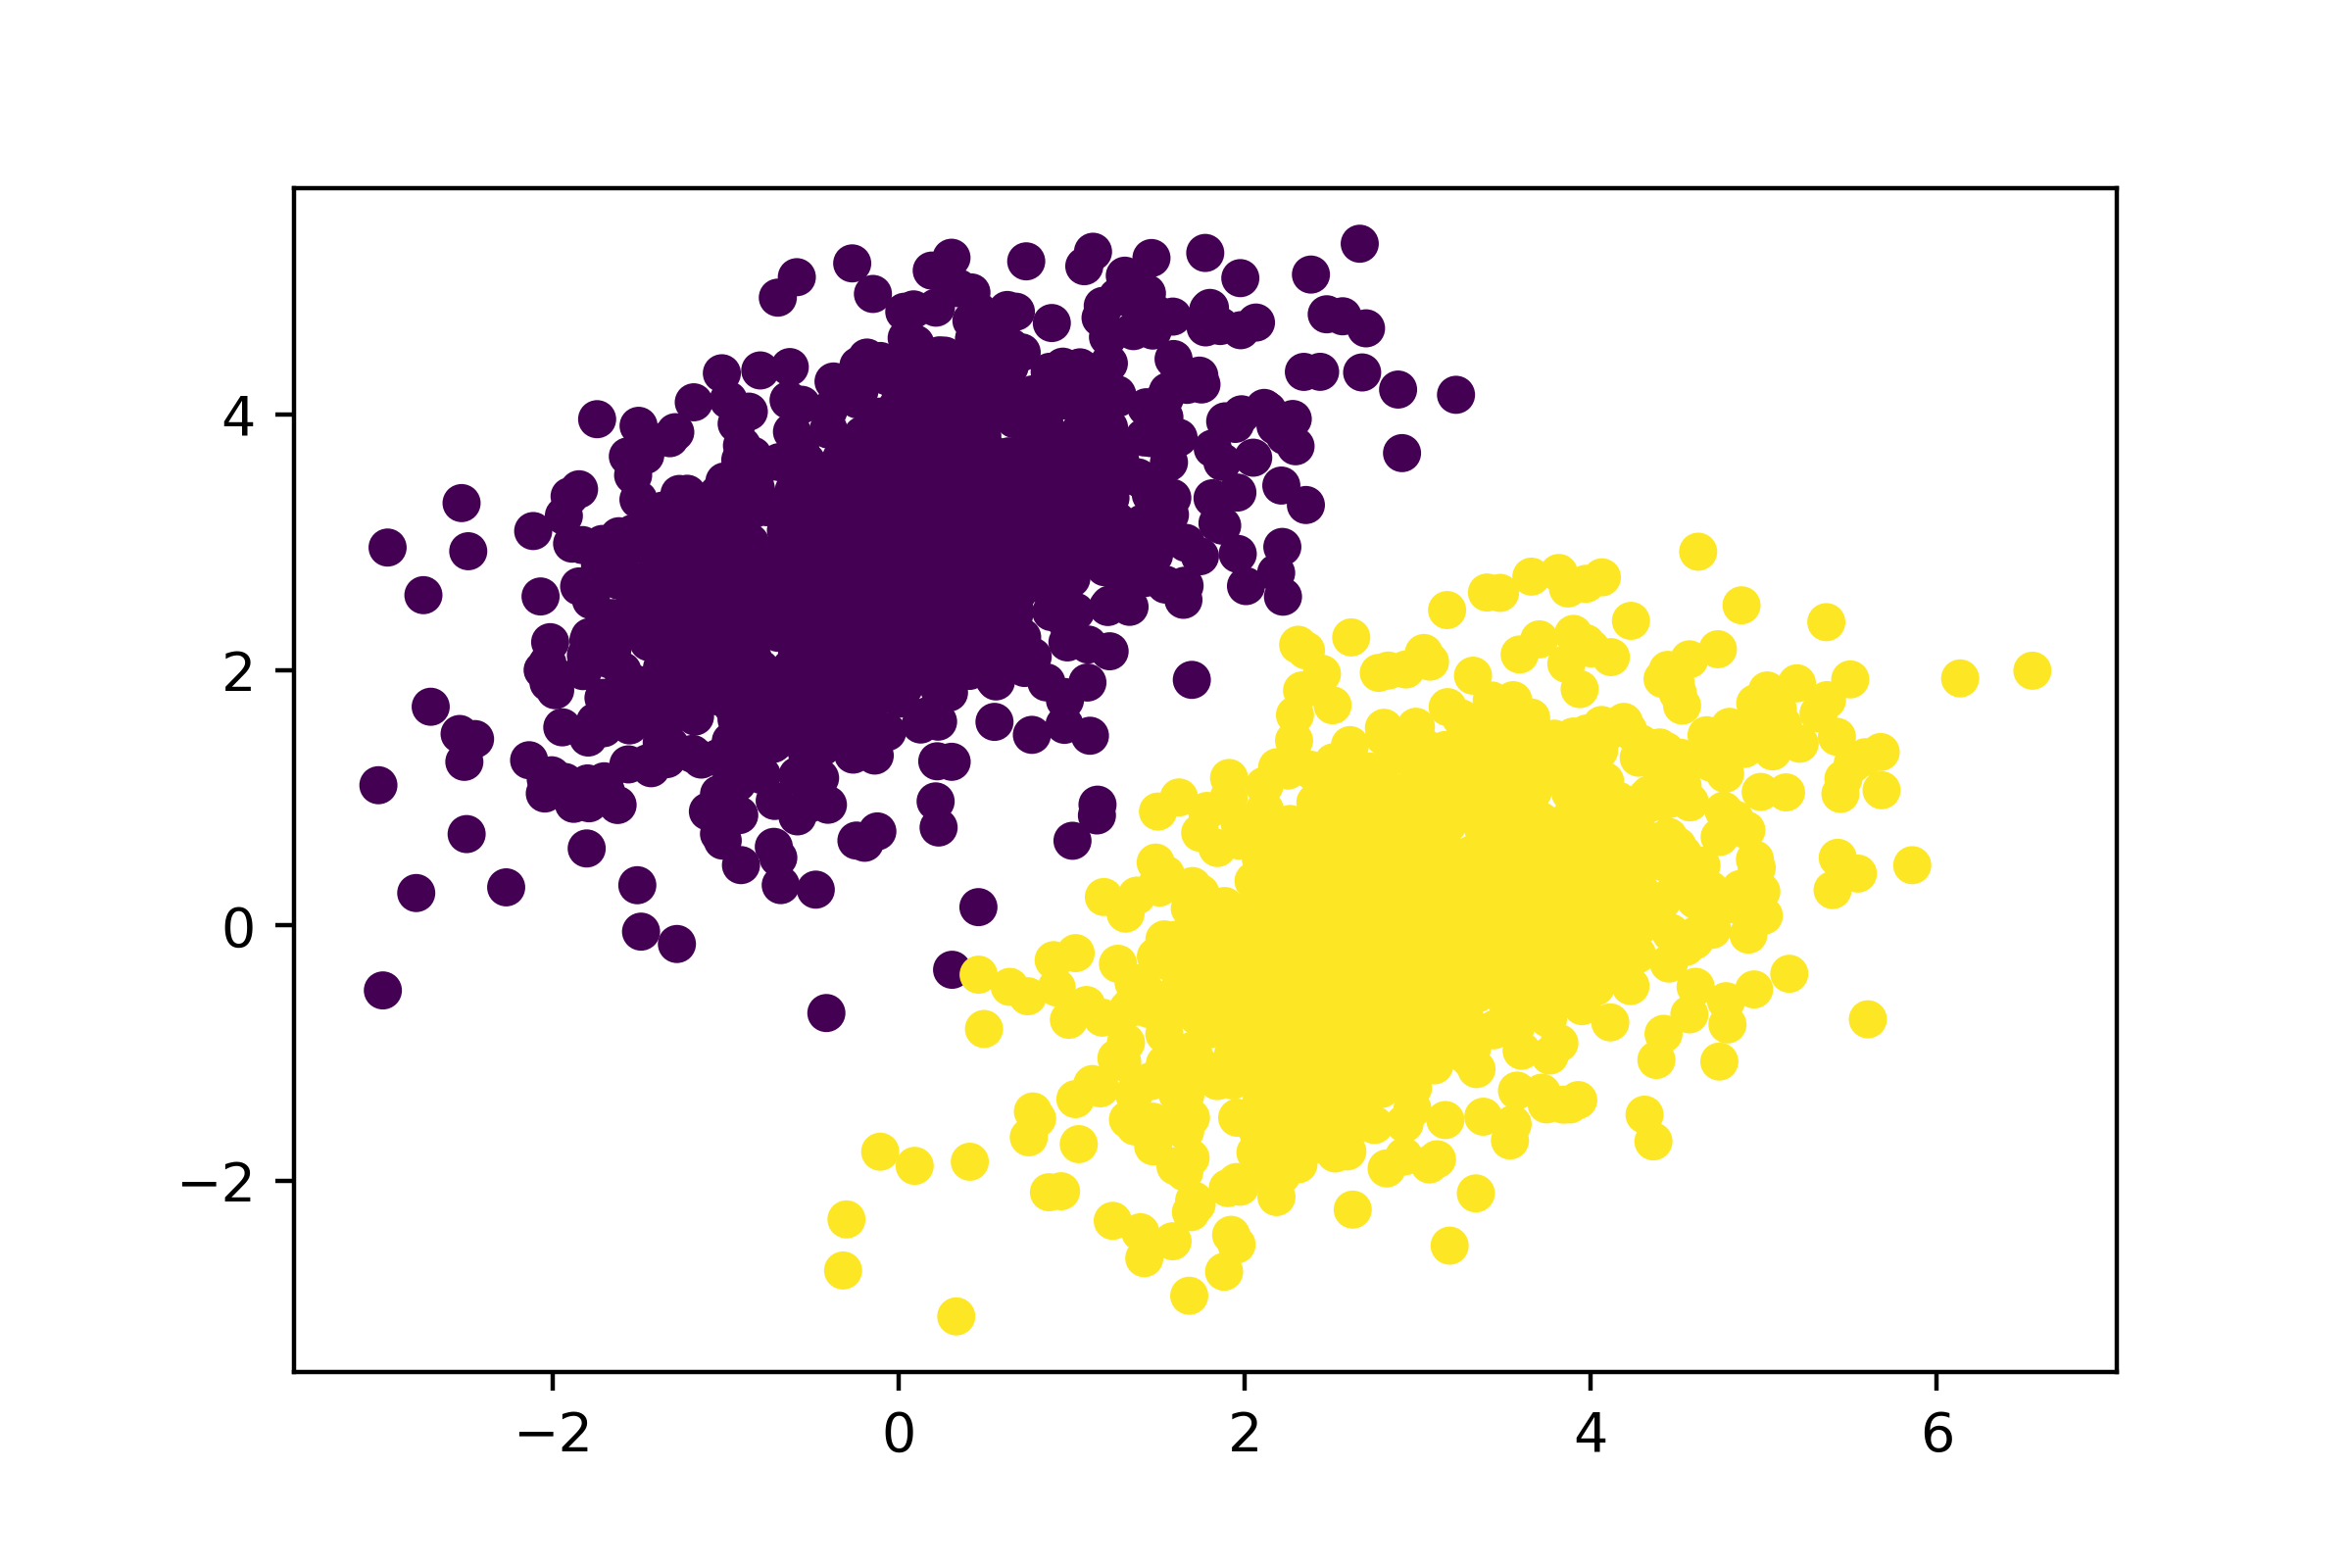
\includegraphics[width=\textwidth,height=0.7\textheight,keepaspectratio]{../../images/ch03/linear_model_predictions.3e5424ac.png}
            \caption{Đường thẳng phân chia trước khi huấn luyện}
        \end{figure}
    \end{columns}
\end{frame}

\begin{frame}[fragile]{Hàm mất mát (MSE) và Vòng lặp huấn luyện}
    Chúng ta cập nhật $\mathbf{W}$ và $\mathbf{b}$ dựa trên đạo hàm:
    \begin{lstlisting}[language=Python]
learning_rate = 0.1
for step in range(40):
    with tf.GradientTape() as tape:
        predictions = tf.matmul(inputs, W) + b
        loss = tf.reduce_mean(tf.square(targets - predictions))
        
    grad_W, grad_b = tape.gradient(loss, [W, b])
    
    W.assign_sub(grad_W * learning_rate)
    b.assign_sub(grad_b * learning_rate)
    \end{lstlisting}
\end{frame}

\begin{frame}{Kết quả sau Vòng lặp huấn luyện}
    \begin{columns}
        \column{0.5\textwidth}
        Sau nhiều bước cập nhật trọng số, bộ phân loại tuyến tính đã tự động xoay và tịnh tiến đường thẳng cắt qua khoảng trống tối ưu.
        \begin{itemize}
            \item Thuật toán Gradient Descent hội tụ!
        \end{itemize}
        
        \column{0.5\textwidth}
        \begin{figure}
            \centering
            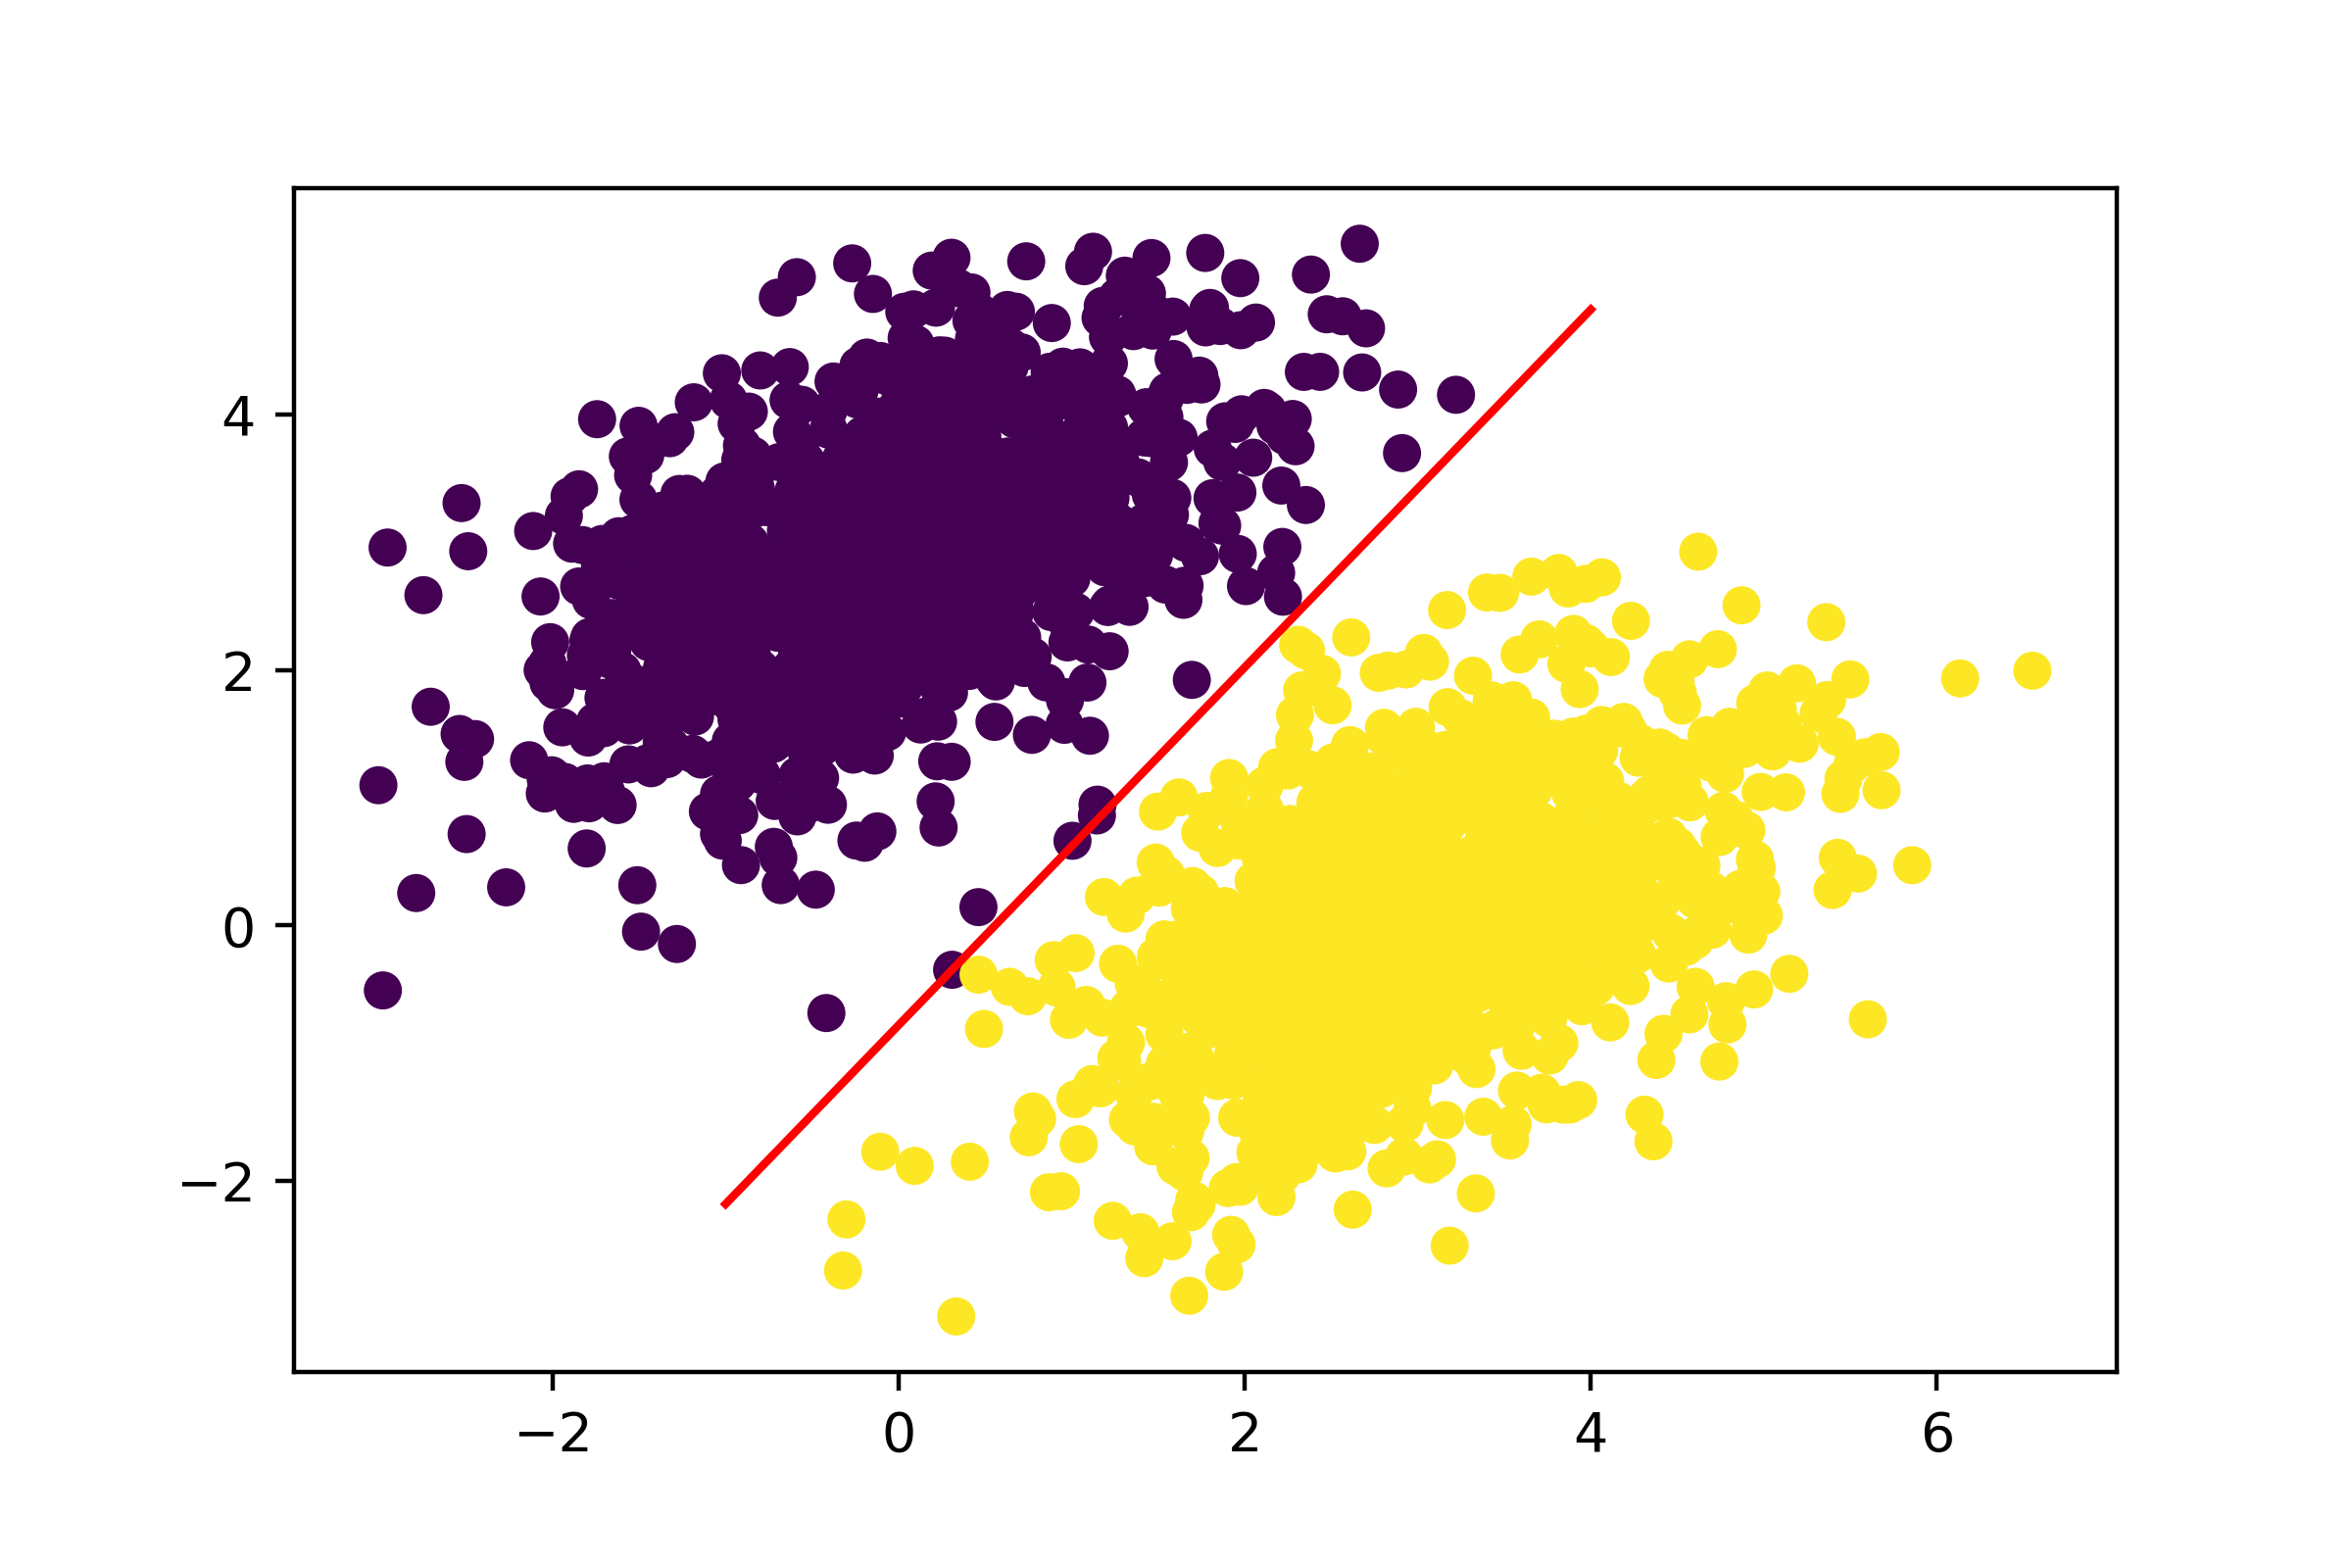
\includegraphics[width=\textwidth,height=0.7\textheight,keepaspectratio]{../../images/ch03/linear_model_with_plotted_line.fd88e7bc.png}
            \caption{Đường thẳng phân chia sau khi huấn luyện}
        \end{figure}
    \end{columns}
\end{frame}

\begin{frame}{Ứng dụng mở rộng: Kiến trúc phức tạp}
    \begin{columns}
        \column{0.5\textwidth}
        \begin{itemize}
            \item Mạng nơ-ron thực tế kết hợp hàng nghìn phép toán $Wx+b$ đan xen với hàm phi tuyến (ReLU, Softmax).
            \item Các kiến trúc khổng lồ như \textbf{Transformer} (mô hình ngôn ngữ) thực chất vẫn sử dụng nguyên lý Backpropagation và Gradient Descent này để học!
        \end{itemize}
        
        \column{0.5\textwidth}
        \begin{figure}
            \centering
            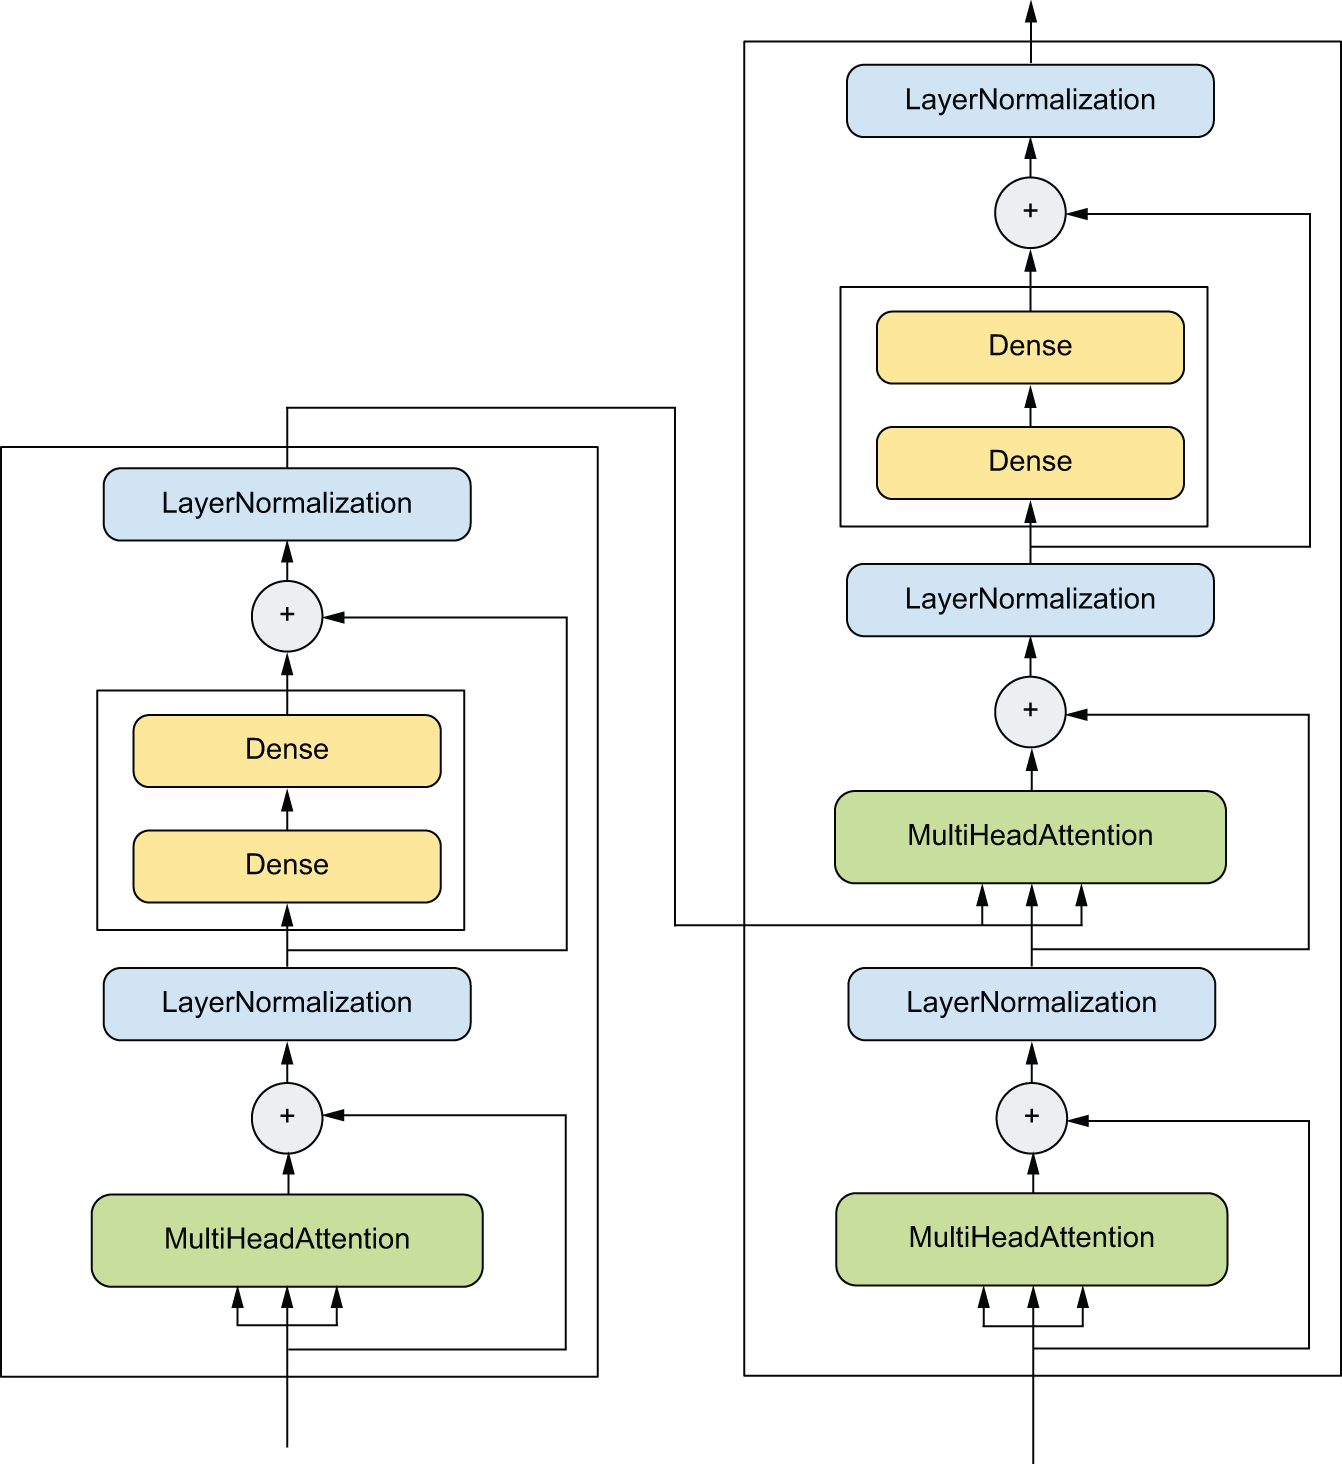
\includegraphics[width=\textwidth,height=0.7\textheight,keepaspectratio]{../../images/ch03/transformer.cb3f137f.png}
            \caption{Đồ thị kiến trúc của Transformer Block}
        \end{figure}
    \end{columns}
\end{frame}

\section{Tổng kết}

\begin{frame}{Tổng kết Chương 3}
    \begin{itemize}
        \item \textbf{TensorFlow, PyTorch, JAX:} 3 "Cột trụ" Framework cung cấp sức mạnh tính toán tự động đạo hàm cực lớn trên GPU/TPU.
        \item \textbf{Keras:} API thượng tầng (High-level) kết nối và chuẩn hóa toàn bộ sự phức tạp của 3 Framework kia thành các khối block (Layers/Models) gọn gàng.
        \item \textbf{Core Logic:} Cho dù 1 lớp Dense hay 1 mô hình Transformer tỷ tham số, bản chất vẫn là Tính Loss $\rightarrow$ Lấy Gradient $\rightarrow$ Cập nhật $W, b$.
    \end{itemize}
\end{frame}

\end{document}
